\chapter{ANALISIS DAN PERANCANGAN}


\section{ANALISIS}

Kegiatan perstatistikan di BPS dilakukan dengan mengacu kepada proses bisnis yang tertuang pada GSBPM. Dalam GSBPM, seperti pada Gambar ~\ref{fig:gsbpm2}, setiap kegiatan perstatistikan dilakukan dalam 8 fase: \textit{Specify needs}, \textit{Design}, \textit{Build}, \textit{Collect}, \textit{Process}, \textit{Analyze}, \textit{Disseminate}, dan \textit{Evaluate}. Tahap \textit{specify needs}, \textit{design}, dan \textit{build} merupakan tahapan-tahapan pada level perencanaan. Tahap \textit{collect} dan \textit{process} merupakan tahapan-tahapan pada level pelaksanaan. Sementara tahap \textit{analyze}, \textit{disseminate}, dan \textit{evaluate} merupakan tahapan-tahapan paska pelaksanaan.


Pada tahap \textit{collect}, data dikumpulkan dengan menggunakan media kuesioner. Sebagian besar kuesioner yang digunakan dalam pengumpulan data di BPS masih menggunakan media kuesioner kertas, meskipun beberapa \textit{survey} telah diujicobakan untuk menggunakan \textit{mobile device}. Sementara pada tahap \textit{process}, kuesioner yang telah terisi pada tahap \textit{collect} dilakukan \textit{editing}, \textit{coding}, dan imputasi. 


\subsection{Penyusunan Model Aplikasi} \label{ssec:analysis-application-model}

Berdasarkan hasil analisis dan studi literatur dari sejumlah pendekatan yang diusulkan, penggunaan \textit{mobile device} sebagai media pengumpulan data dapat diimplementasikan dalam beberapa mekanisme:

\begin{enumerate}
\item \hyperref[sssec:stand-alone]{Pendekatan \textit{stand alone}}
\item \hyperref[sssec:client-server]{Pendekatan \textit{client server}}
\item \hyperref[sssec:client-server-proxy]{Pendekatan \textit{client server} dengan \textit{proxy}}
\end{enumerate}


\subsubsection{Pendekatan \textit{Stand Alone}} \label{sssec:stand-alone}

Pendekatan \textit{stand alone} merupakan model dimana data didistribusikan pada \textit{device}. Pada pendekatan ini \textit{client application} dan data diletakkan pada \textit{device} yang sama. Sementara itu, pada \textit{central server} terdapat database yang memuat seluruh master dan kompilasi data dari keseluruhan \textit{device}. Untuk memastikan kedua sisi, baik \textit{device} maupun \textit{central server}, memuat data yang sama, maka terdapat replikasi dan sinkronisasi yang menghubungkan keduanya. Replikasi dan sinkronisasi dilakukan oleh \textit{sync client} pada sisi \textit{device}, yang berkomunikasi dengan \textit{sync server} pada sisi \textit{central server}. Gambar ~\ref{fig:design-stand-alone} merupakan ilustrasi cara kerja pendekatan \textit{stand alone}, sementara Gambar ~\ref{fig:design-stand-alone-flowchart} menunjukkan alur kerja dari pendekatan \textit{stand alone}.

\begin{figure}[h]
    \centering
    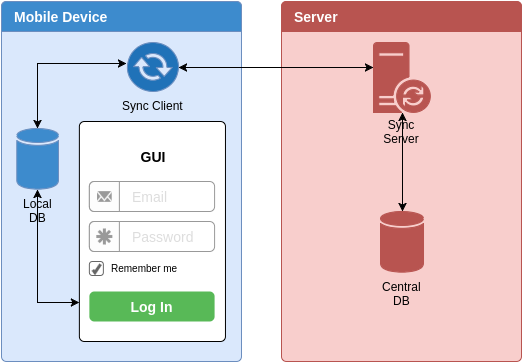
\includegraphics[width=.7\textwidth]{../../Resources/Images/design-stand-alone}
    \caption{Pendekatan \textit{Stand Alone}}
    \label{fig:design-stand-alone}
\end{figure}

\begin{figure}[h]
    \centering
    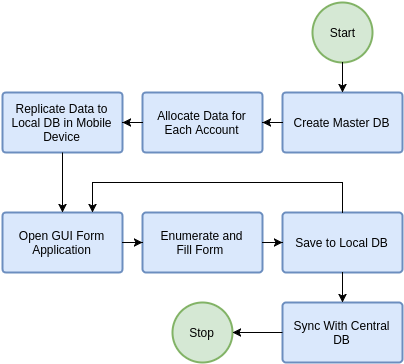
\includegraphics[width=.7\textwidth]{../../Resources/Images/design-stand-alone-flowchart}
    \caption{\textit{Flowchart} Pendekatan \textit{Stand Alone}}
    \label{fig:design-stand-alone-flowchart}
\end{figure}

Sinkronisasi data pada pendekatan \textit{stand alone} mempunyai karakteristik sebagai berikut:
\begin{enumerate}
\item Sinkronisasi menggunakan \textit{scheduler} yang akan di-\textit{trigger} setiap periode waktu tertentu
\item \textit{Event listener} digunakan untuk mendeteksi status dari \textit{device}, apakah dalam kondisi \textit{connected} maupun \textit{disconnected}. Pada saat \textit{device} berubah \textit{state} dari \textit{disconnected} menjadi \textit{connected}, maka sinkronisasi akan di-\textit{trigger} tanpa menunggu \textit{schedule}.
\end{enumerate}

Keuntungan dari pendekatan \textit{stand alone} adalah \textit{latency} yang terjadi pada saat \textit{client application} mengakses data menjadi lebih kecil dikarenakan letak data berada pada \textit{local machine}. Selain itu, pendekatan ini juga dapat digunakan pada \textit{disconnected environment}, dimana untuk kasus pengumpulan data lapangan kondisi ini akan sering dijumpai. Sementara itu, kelemahan pendekatan \textit{stand alone} ada pada letak eksekusi validasi yang terdapat pada sisi \textit{client}, sehingga perbaikan \textit{rule} validasi harus diikuti dengan pembaharuan aplikasi.


\subsubsection{Pendekatan \textit{Client Server}} \label{sssec:client-server}

Pendekatan \textit{client server} merupakan pendekatan tersentral, dimana data terletak pada tempat yang berbeda dengan \textit{client application}, sebagaimana Gambar ~\ref{fig:design-client-server}. Sementara Gambar ~\ref{fig:design-client-server-flowchart} menunjukkan alur kerja dari pendekatan \textit{client server}.


Jika pada pendekatan \textit{stand alone} diperlukan suatu mekanisme pendistribusian data pada masing-masing \textit{account/device} dengan replikasi dan sinkronisasi, maka pada pendekatan \textit{client server} hal tersebut tidak diperlukan. Kondisi dimana hanya ada server tunggal dan data yang tersentralisasi memiliki konsekuensi data akan selalu konsisten. Selain itu, pembaharuan aplikasi juga dapat diminimalisir dengan menempatkan rule validasi pada sisi server.


Kelemahan yang dimiliki pendekatan \textit{client server} adalah, untuk dapat digunakan, \textit{client application} harus selalu terkoneksi dengan \textit{central server} dimana data berada, seperti Gambar ~\ref{fig:design-client-server-flowchart}, sehingga pendekatan ini tidak dapat digunakan pada \textit{disconnected environment}. Selain itu, setiap kali \textit{client application} melakukan komunikasi dengan \textit{central server}, maka sejumlah data akan ditransmisikan, sehingga diperlukan kapasitas dan kapabilitas jaringan yang cukup baik kuota maupun \textit{transfer rate}. 

\begin{figure}[h]
    \centering
    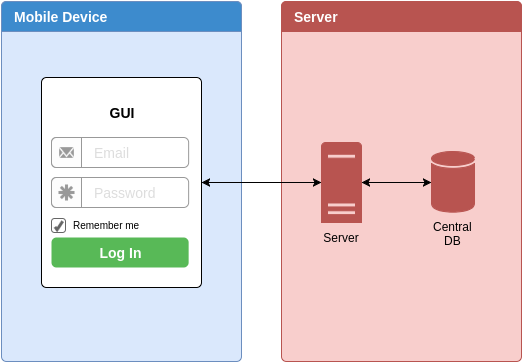
\includegraphics[width=.7\textwidth]{../../Resources/Images/design-client-server}
    \caption{Pendekatan \textit{Client Server}}
    \label{fig:design-client-server}
\end{figure}

\begin{figure}[h]
    \centering
    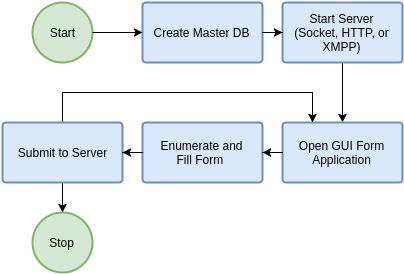
\includegraphics[width=.7\textwidth]{../../Resources/Images/design-client-server-flowchart}
    \caption{\textit{Flowchart} Pendekatan \textit{Client Server}}
    \label{fig:design-client-server-flowchart}
\end{figure}


\subsubsection{Pendekatan \textit{Client Server} dengan \textit{Proxy}} \label{sssec:client-server-proxy}

Pendekatan \textit{client server} dengan \textit{proxy} menggunakan sebuah \textit{proxy server} yang diletakkan antara \textit{client application} dan \textit{central server}. \textit{Proxy server} disini berperan sebagai \textit{Application-Level Gateway (ALG)} yang menyediakan fungsi \textit{security}, \textit{filtering}, dan \textit{packet forwarding}. Seperti pada Gambar ~\ref{fig:design-client-server-proxy}, \textit{proxy server} diletakkan pada sisi \textit{client/device}, dan akan mewakili \textit{client application} dalam berkomunikasi dengan \textit{server}.


Dari sisi \textit{client}, pendekatan \textit{client server} dengan \textit{proxy} memiliki cara kerja yang mirip dengan pendekatan \textit{stand alone}, yaitu data terdistribusi pada \textit{device}, sehingga \textit{client application} dan data terletak pada \textit{device} yang sama.

\begin{figure}[h]
    \centering
    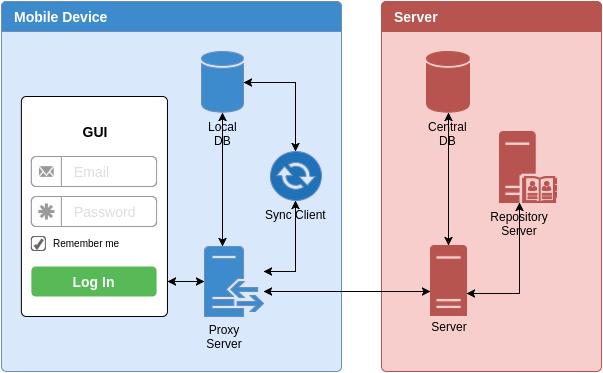
\includegraphics[width=.8\textwidth]{../../Resources/Images/design-client-server-proxy}
    \caption{Mekanisme \textit{Client Server} dengan \textit{Proxy}}
    \label{fig:design-client-server-proxy}
\end{figure}

\textit{Proxy} dalam konteks ini, selain mengacu kepada \textit{proxy server} juga mengacu kepada konsep \textit{proxy} dalam hal pemrograman. \textit{Proxy} dalam pemrograman ini memungkinkan implementasi dari \textit{interface} di-\textit{load} pada saat \textit{runtime}, seperti \textit{class reflection} dan \textit{method invocation}. Salah satu contoh implementasi \textit{proxy} dalam pemrograman adalah \textit{class Proxy} yang terdapat pada \textit{Java Refrection API}.


\textit{Proxy} dalam hal pemrograman digunakan untuk mereplikasi \textit{rule} validasi yang ditulis dalam suatu bahasa pemrograman tertentu. Replikasi \textit{rule} validasi dimaksudkan untuk memperbarui \textit{rule} validasi yang digunakan dari sisi \textit{client}. Pendekatan ini memungkinkan pengeksekusian \textit{rule} validasi dilakukan secara terpisah dari \textit{client application}, sehingga pembaruan \textit{rule} validasi-pun dapat dilakukan secara \textit{independent} tanpa memperbarui \textit{client application}.


Berdasarkan analisis terhadap kebutuhan dalam pengumpulan data dengan menggunakan \textit{mobile device}, maka desain yang dirancang harus mempertimbangkan kriteria berikut:

\begin{enumerate}
\item Mendukung \textit{disconnected environment} \\
Pengumpulan data memerlukan penyisiran lapangan dengan kondisi geografis yang bervariasi. Kondisi sinyal telekomunikasi pada masing-masing wilayah pendataan juga bervariasi, dari yang bagus sampai yang tidak terdapat sinyal komunikasi. Desain yang dirancang harus dapat mengakomodir pengumpulan data pada wilayah yang tidak terdapat sinyal komunikasi.

\item Mendukung pembaharuan secara otomatis \\
Kuesioner elektronik yang terinstal pada \textit{device} merupakan representasi dari variabel sensus/survei yang akan dikumpulkan. Dalam pengisiannya, ada aturan \textit{rule} validasi yang harus diikuti, sehingga pembaharuan \textit{rule} validasi diperlukan ketika ada perbaikan konsep dan definisi.
\end{enumerate}

Oleh karena itu, berdasarkan kriteria-kriteria tersebut, penggunaan pendekatan \hyperref[sssec:client-server-proxy]{\textit{client server} dengan \textit{proxy}} dapat memenuhi kriteria yang dibutuhkan, yaitu: dapat digunakan pada \textit{disconnected environment} melalui \textit{packet forwarding} dan mendukung pembaharuan secara otomatis melalui \textit{dynamic class loading}.


\subsection{Pengelolaan Data}

Pada tahap analisis \hyperref[ssec:analysis-application-model]{penyusunan model aplikasi} diperoleh kesimpulan bahwa pendekatan \hyperref[sssec:client-server-proxy]{\textit{client server} dengan \textit{proxy}} adalah yang paling sesuai dengan kebutuhan. Pada pendekatan tersebut, terdapat 2 (dua) jenis penyimpanan data, yaitu pada sisi \textit{client} dan sisi \textit{server}. Agar kedua sisi penyimpanan data tersebut merepresentasikan data yang sama, maka terdapat mekanisme pengelolaan data yang harus diikuti.

Dalam kegiatan pengumpulan data lapangan, terdapat 2 (dua) jenis data yang digunakan:

\begin{enumerate}
\item Data \textit{master} \\
Data \textit{master} merupakan data yang digunakan sebagai referensi oleh variabel pendataan. Data \textit{master} bersifat \textit{non-volatile}, yang artinya tidak mudah berubah. Perubahan data master hanya dapat dilakukan pada \textit{phase} design pada GSBPM. Contoh data \textit{master} antara lain: data master wilayah, data master status perkawinan, data master status dalam rumah tangga, dll.

\item Data lapangan \\
Data lapangan merupakan data yang isinya merupakan representasi hasil pendataan. Data ini bersifat transaksional, artinya data dapat dengan mudah ditambah, dihapus, maupun di\textit{update}. Contoh data lapangan antara lain: data sakernas semester I 2016, data susenas semester I 2016, data usaha rumah tangga pertanian ST2016, dll.
\end{enumerate}


Secara umum, variabel yang sejenis yang digunakan pada beberapa sensus maupun survei mempunyai konsep dan definisi yang sama, misalnya: Variabel jenis kelamin pada Sakernas \footnote{\url{https://sirusa.bps.go.id/index.php?r=variabel/view&id=11482}}, Susenas \footnote{\url{https://sirusa.bps.go.id/index.php?r=variabel/view&id=12526}}, SUPAS \footnote{\url{https://sirusa.bps.go.id/index.php?r=variabel/view&id=11341}}, dll, mempunyai konsep dan definisi, serta atribut yang sama, yaitu: 1 - laki-laki, 2 - perempuan. Begitu pula variabel-variabel yang lain, digunakan secara bersamaan oleh beberapa sensus dan survei.


Dari hasil analisis berdasarkan jenis-jenis data dan karakteristik variabel yang digunakan, maka dapat dirangkum dalam beberapa poin berikut:

\begin{enumerate}
\item \textit{Server} memuat seluruh data \textit{master} yang digunakan pada seluruh kegiatan sensus dan survei.
\item \textit{Client} memuat hanya data \textit{master} yang digunakan oleh kegiatan tertentu sana.
\item Data \textit{master} bersifat \textit{non-volatile}, sehingga diasumsikan data master pada \textit{server} lebih \textit{up-to date} dibandingkan data master pada \textit{client}. Oleh karena itu, replikasi data \textit{master} dilakukan dari \textit{server} ke \textit{client}.
\item Data lapangan bersifat transaksional, artinya data lapangan pada \textit{client} diasumsikan kondisinya lebih \textit{up-to date} dibandingkan data lapangan pada \textit{server}. Oleh karena itu, replikasi data lapangan dilakukan dari \textit{client} ke \textit{server}.
\end{enumerate}


\section{PERANCANGAN}

Secara garis besar, terdapat 2 (dua) jenis \textit{object} yang menjadi poin utama dari solusi yang akan dirancang, yaitu: data dan \textit{rule} validasi. Gambar ~\ref{fig:architecture-solution} menunjukkan arsitektur dari solusi yang akan dirancang. Terdapat 3 (tiga) mekanisme yang diadopsi pada rancangan solusi: Replikasi, Sinkronisasi, dan  \textit{Routing}.

\begin{figure}[h]
    \centering
    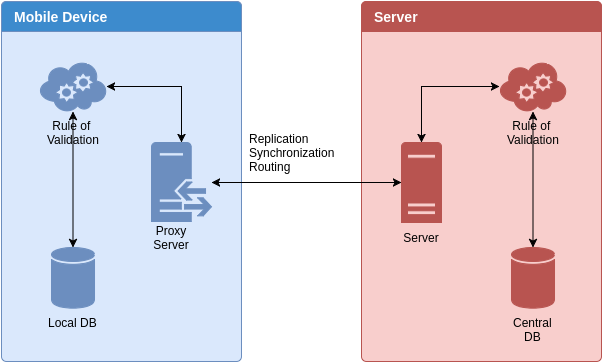
\includegraphics[width=.87\textwidth]{../../Resources/Images/architecture-solution}
    \caption{Arsitektur Solusi}
    \label{fig:architecture-solution}
\end{figure}


\subsection{Replikasi}

Replikasi merupakan suatu cara untuk memastikan agar baik \textit{device} maupun \textit{server} mengeksekusi objek yang sama. Replikasi dilakukan satu arah, yaitu dari \textit{server} ke \textit{device}. Terdapat 2 (dua) jenis mekanisme replikasi yang dirancang, yaitu: replikasi rule dan replikasi data.


\subsubsection{Replikasi \textit{Rule} Validasi}

\textit{Rule} validasi ada implementasi dari \textit{logic workflow}, seperti yang tertuang pada GSBPM fase \textit{Build} subproses \textit{Configure Workflows}. Replikasi \textit{rule} validasi bertujuan agar validasi isian kuesioner dapat dijalankan secara lokal. Implementasi \textit{rule} validasi dikemas dalam bentuk \textit{OSGI Bundle}.


\subsubsection{Replikasi Data}

\textit{Rule} validasi selain memuat \textit{logic workflow} juga memuat \textit{object} yang merupakan representasi dari tabel di \textit{database} yang disebut \textit{Object Relational Mapping (ORM)}. ORM inilah yang akan menentukan tabel dan data apa saja yang akan di replikasi.


\subsection{Sinkronisasi}

Seperti halnya replikasi, sinkronisasi juga bertujuan untuk memastikan \textit{device} dan \textit{server} mengeksekusi objek yang sama. Akan tetapi, sinkronisasi berjalan sepanjang waktu, baik melalui \textit{scheduler} maupun \textit{trigger}. Selain itu, sinkronisasi dilakukan dua arah, dari \textit{server} ke \textit{device} maupun dari \textit{device} ke \textit{server}, tergantung \textit{object} yang sedang dieksekusi.


\subsubsection{Sinkronisasi \textit{Rule} Validasi}

Sinkronisasi \textit{rule} validasi menggunakan implementasi yang sama dengan replikasi \textit{rule} validasi. Perbedaanya, sinkronisasi \textit{rule} validasi menggunakan \textit{trigger} yang berupa versi. Setiap kali \textit{client application} menemukan pembaharuan versi \textit{rule} validasi pada server, maka \textit{client application} secara otomatis akan memperbarui \textit{rule} validasinya.


\subsubsection{Sinkronisasi Data}

Sebagaimana yang telah dijabarkan dalam analisis, terdapat 2 (dua) jenis data yang dikelola, yaitu: data \textit{master} dan data lapangan. Arah sinkronisasi data menyesuaikan jenis data-nya. Data master pada \textit{server} diasumsikan lebih \textit{up-to-date}, sehingga sinkronisasi dilakukan dari arah \textit{server} ke \textit{device}. Sebaliknya, data lapangan pada \textit{device} diasumsikan lebih \textit{up-to-date}, sehingga sinkronisasi dilakukan dari arah \textit{device} ke \textit{server}.


\subsection{Routing}

Proses \textit{routing} menggunakan sebuah \textit{proxy server}. \textit{Proxy server} berperan sebagai \textit{Application-Level Gateway (ALG)} yang menyediakan fungsi \textit{security}, \textit{filtering}, dan \textit{packet forwarding}. 
